\section{Tool Support and Future Work}
\label{sec:toolsupport}
\subsection{Assurance Case Modelling Environment - ACME}
With all its power in model-based system assurance, there is one drawback of SACM, which is the lack of concrete syntax, i.e. graphical representations of SACM. 
Without graphical representations, it is typically difficult for engineers to construct SACM. 
Hence, in order to exploit the benefits provided by SACM, we implement a tool (Assurance Case Modelling Environment, ACME\footnote{Available upon request.}) based on the GSN metamodel we discussed in Section~\ref{sec:mapping}. 

\begin{figure}
	\centering
	\begin{minipage}[b]{0.49\textwidth}
		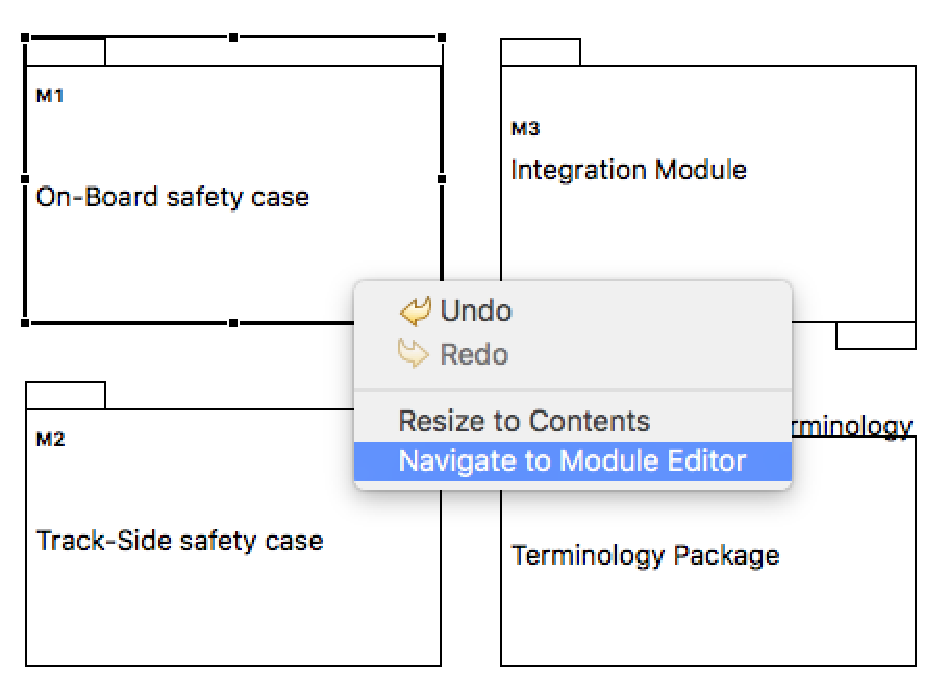
\includegraphics[width=1\linewidth]{ac_view.pdf}
		\caption{The Assurance Case Package View of ACME.}
		\label{fig:ac_view}
	\end{minipage}
	\hfill
	\begin{minipage}[b]{0.49\textwidth}
		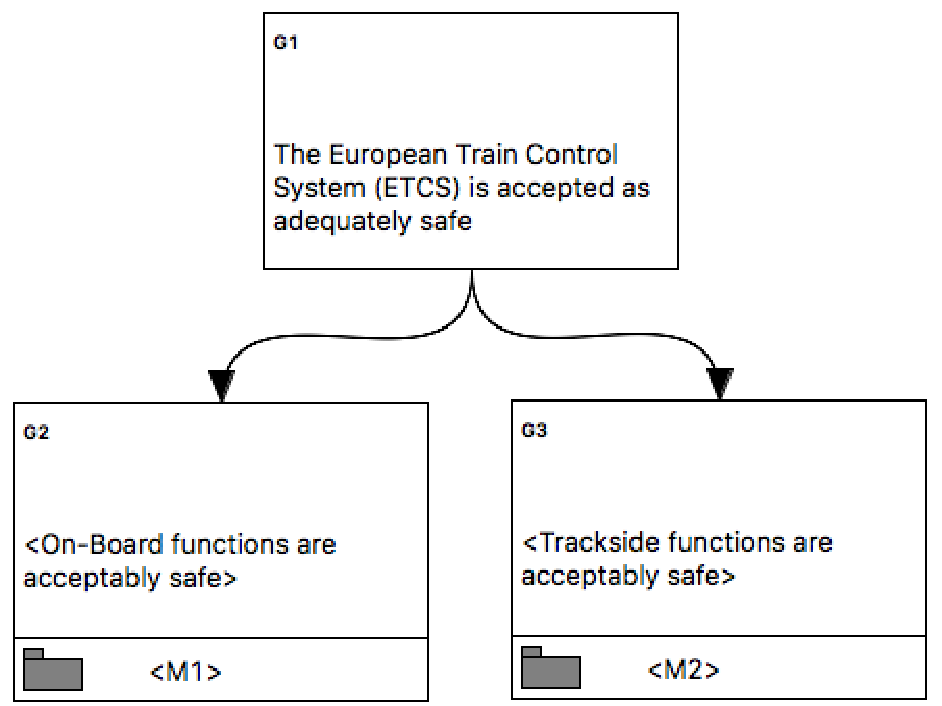
\includegraphics[width=\textwidth]{module_view.pdf}
		\caption{The Module View of ACME.}
		\label{fig:module_view}
	\end{minipage}
\end{figure}

\begin{figure}
	\centering
	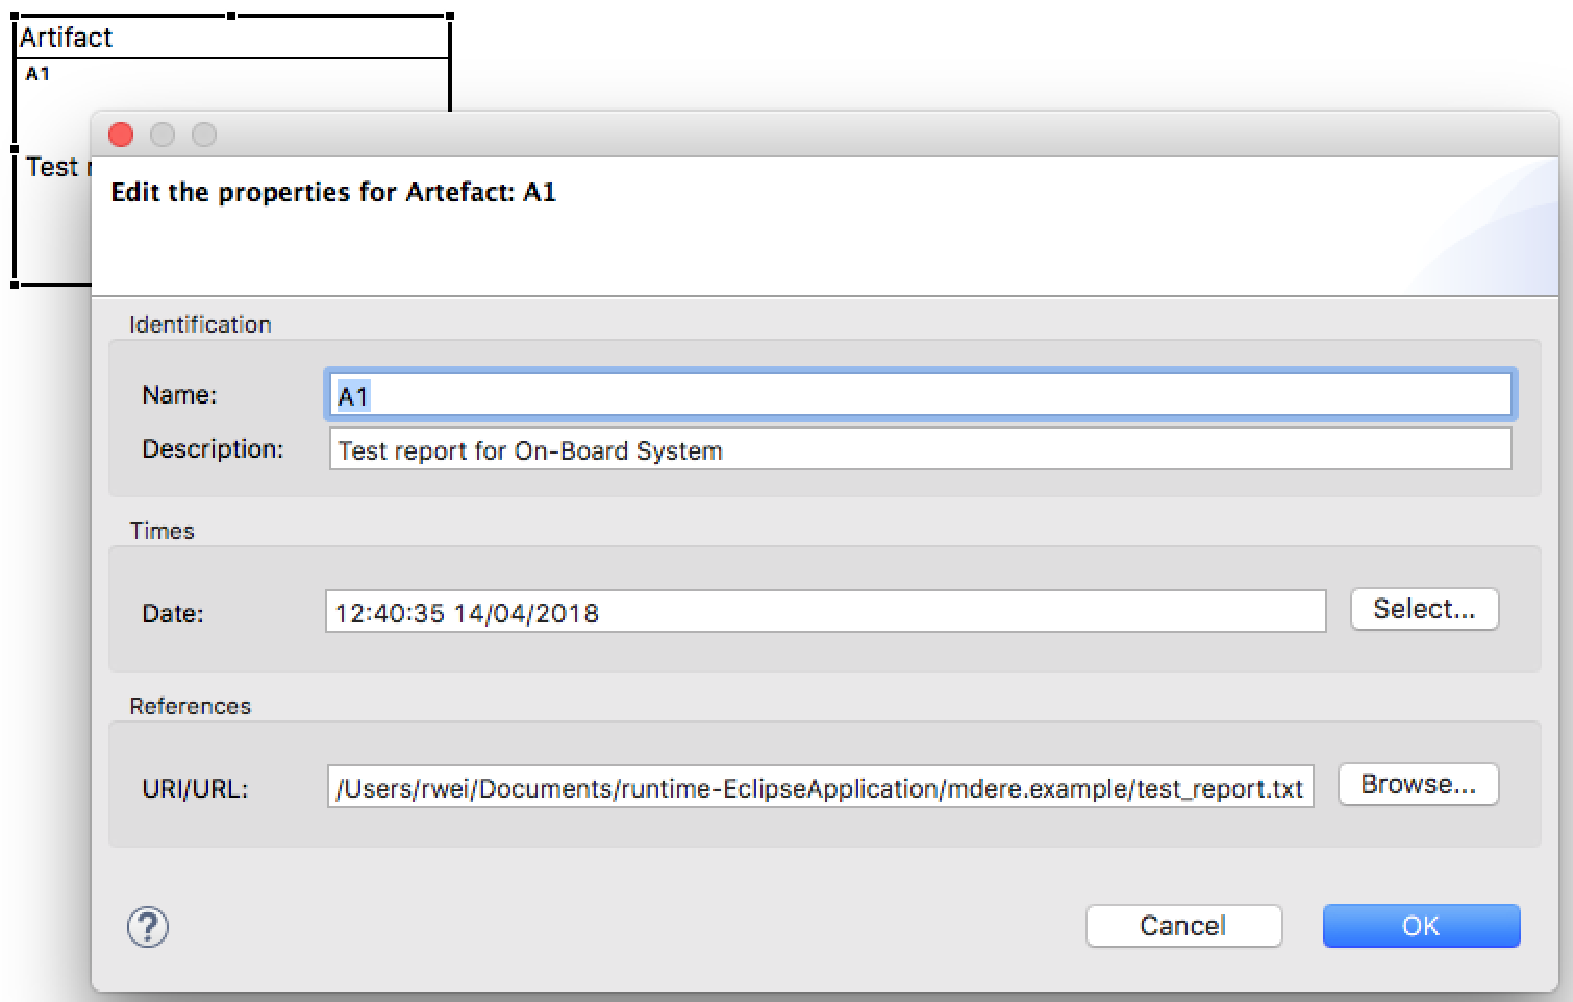
\includegraphics[width=1\linewidth]{artifact_view.pdf}
	\caption{Creation of Artifact.}
	\label{fig:artifact_view}
\end{figure}

\begin{figure}
	\centering
	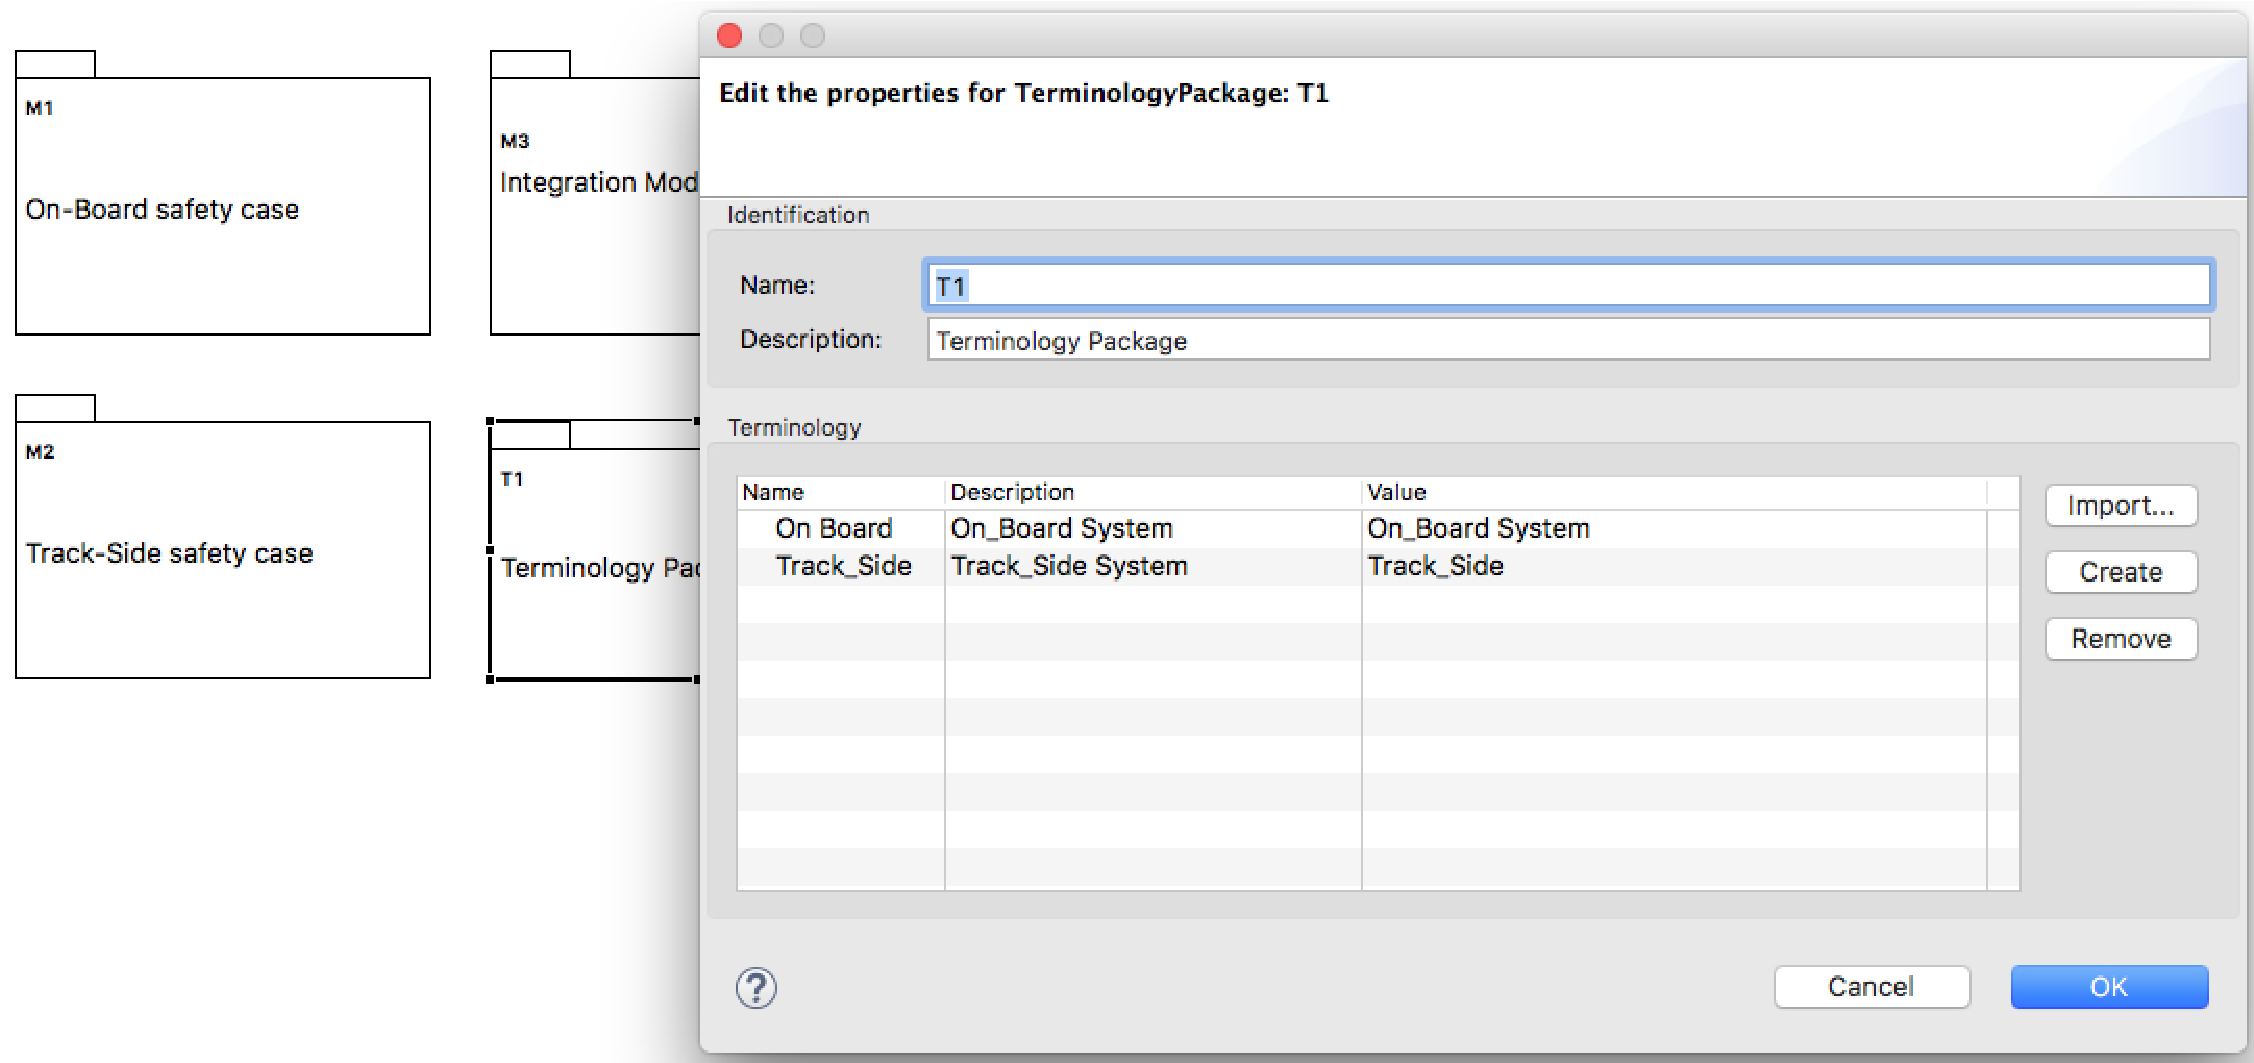
\includegraphics[width=1\linewidth]{terminology_view.pdf}
	\caption{Editing a \textit{TerminologyPackage}.}
	\label{fig:terminology_view}
\end{figure}

ACME is implemented using the Graphical Modelling Framework (GMF) \cite{gmf}, which supports the creation of editors based on metamodels defined using the Ecore metamodel provided by the Eclipse Modelling Framework (EMF) \cite{steinberg2008emf}. 
As previously discussed, the GSN metamodel inhertis all elements in the SACM metamodel, which means that the users of ACME are able to create GSN elements as well as elements inherited from SACM.

Figure~\ref{fig:ac_view} shows the Assurance Case Package View, within which the users are able to create Modules and Contract Modules of GSN, as well as elements defined in the \textit{AssuranceCase} package of SACM. 
Figure~\ref{fig:module_view} shows the Module view of ACME, where the users are able to create GSN elements. 

The users are also able to create elements in the \textit{Artifact} package (i.e. \textit{Artifact}, \textit{Activity}, \textit{Event}, \textit{Participant}, \textit{Technique}, \textit{Resource}, \textit{Property}, and \textit{ArtifactAssetRelationship}), Figure~\ref{fig:artifact_view} demonstrates how an \textit{Artifact} can be created/edited. 
Creation tools are also provided for the elements in the \textit{Terminology} package, where a \textit{TerminologyPackage} is represented as a table in ACME, Figure~\ref{fig:terminology_view} demonstrates how a \textit{TerminologyPackage} and its contents can be created/edited.

ACME eases the creation of assurance cases in the sense that the argumentation made in the assurance case can be modelled using GSN which system assurance engineers are more familiar with (in the sense that the models produced by ACME conform to the GSN metamodel described in Section~\ref{sec:mapping}). 
In addition, based on the transformation from GSN to SACM, ACME provides a conversion mechanism, where the created GSN model using ACME can be transformed into a SACM model, with the help of model-to-model transformation (implemented in Epsilon Transformation Language \cite{kolovos2008epsilon}), as shown in Figure~\ref{fig:transformation_view}.

\begin{figure}
	\centering
	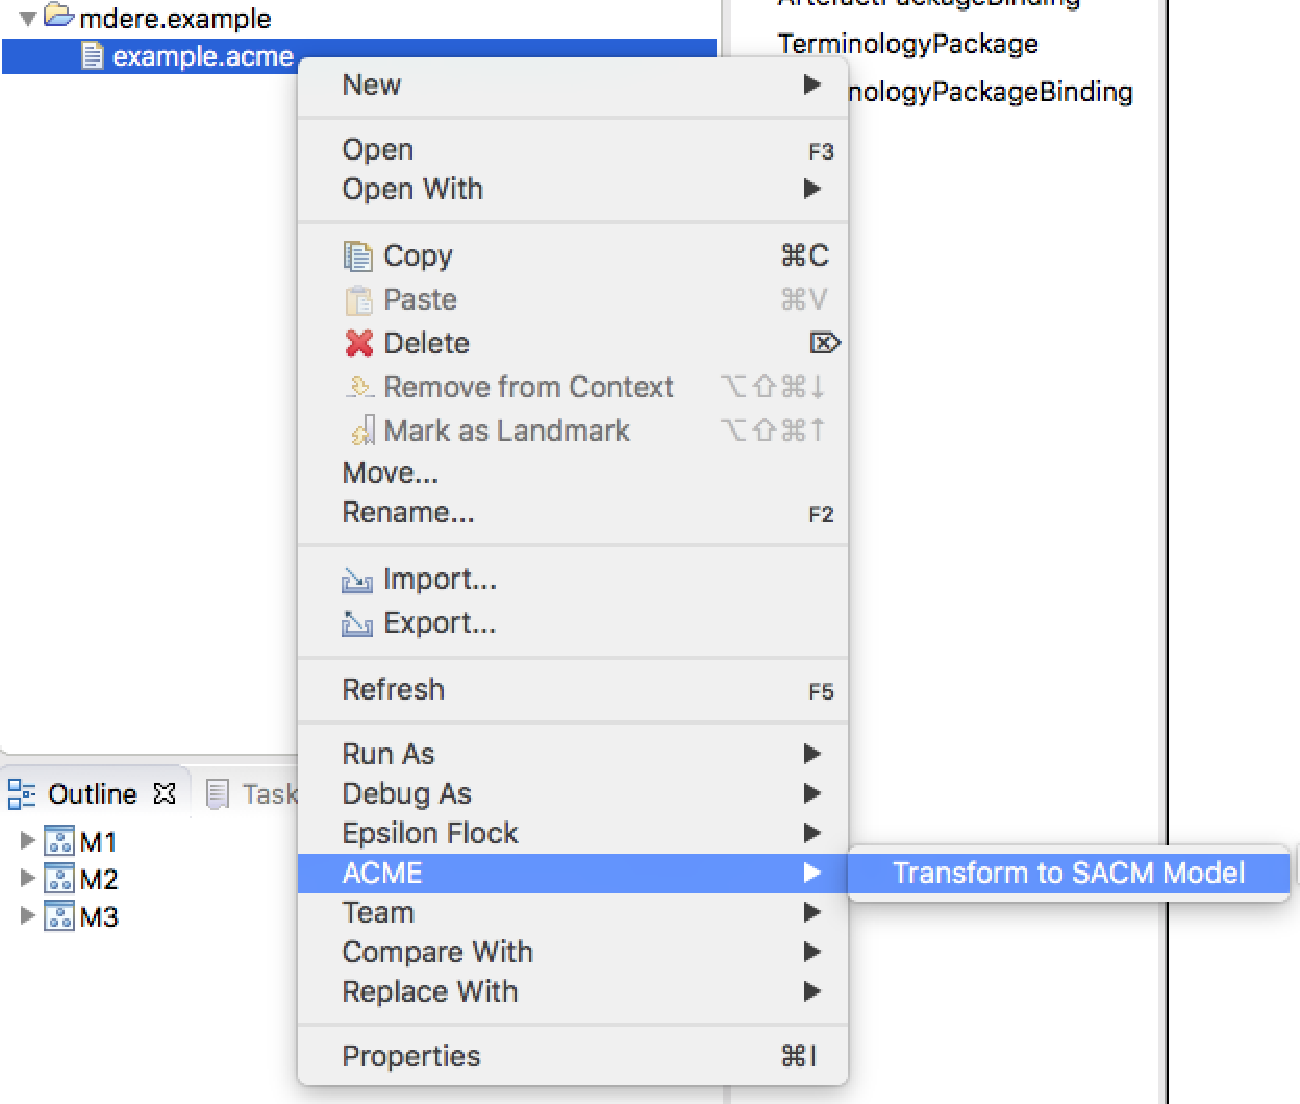
\includegraphics[width=1\linewidth]{gsn2sacm_view.pdf}
	\caption{M2M function provided by ACME to transform a GSN model to a SACM model.}
	\label{fig:transformation_view}
\end{figure}

ACME provides a transitional solution to model-based system assurance in the sense that it enables GSN users to fully exploit the potentials of SACM whilst being able to adopt the tool with their existing knowledge in using GSN. 

\subsection{Future Work}
With regard to future work, our priority will focus on the support of importing legacy GSN/CAE models created by other drawing tools, typically those that can be consumed by computers but are not model-based. 
ACME integrated the Epsilon platform\footnote{\url{https://www.eclipse.org/epsilon/}} with it, which provides a set of extensible model management languages, as well as extensible support for models defined in various formats.
Thus, as long as legacy GSN/CAE models can be consumed by computers, corresponding \textit{driver}s can be created for the Epsilon platform to process such artefacts and transform them into GSN/SACM models via chaining transformations.

To the best of our knowledge, OMG is attempting to standardise the concrete syntax for SACM, we will provide support to the concrete syntax in ACME by creating Argumentation editors for SACM's \textit{Argumentation} package. 
We will also investigate automated model validation to validate GSN/SACM models which has not been investigated before. We have not provided support for instantiating argumentation patterns, we will investigate the use of \textit{ImplementationConstraint}s for pattern instantiation.